% !TEX root =  ../main_manuscript.tex 
\section{Demonstration of Personalized Schedules}
\label{sec:results}
To demonstrate the application of personalized schedules \textcolor{Red}{\st{on real patients}}, \textcolor{Green}{we return to the problem of scheduling biopsies in prostate cancer active surveillance study, PRIAS, described in Section~\ref{sec:introduction}}. The current PRIAS protocol for biopsies is fixed biopsies at year one, four, seven, and ten of follow-up, and every five years after that. Additional annual biopsies are scheduled if a patient's PSA doubling-time~\citep{bokhorst2015compliance} is high. The PSA is measured quarterly for the first two years, and semi-annually after that. The DRE is also measured semi-annually. \textcolor{Green}{The dataset} \textcolor{Red}{\st{is summarized}} \textcolor{Green}{summary from \citet{tomer2020webapp} is also provided Web-Appendix~B}.

The clinical data in PRIAS consists of longitudinal PSA (continuous: ng/mL) and DRE (binary: tumor palpable or not) measurements, patient age at baseline, history of biopsies, and interval-censored times of cancer progression. The event of interest is cancer progression. \textcolor{Green}{We aim to utilize the model definition from a joint model fitted previously to the PRIAS dataset~\citep{tomer2019personalized}, to further create personalized biopsy schedules in new PRIAS patients.}

\subsection{Joint Model Fitted to the PRIAS Dataset}
In the joint model fitted to the PRIAS dataset, PSA was $\log_2(\mbox{PSA} + 1)$ transformed and cancer progression was the event of interest (Web-Appendix~B.3). For PSA, a linear mixed-effects sub-model, wherein PSA profiles are modeled non-linearly over follow-up using B-splines~\citep{de1978practical} was utilized. For DRE, a logistic mixed-effects sub-model was utilized. To link the PSA and DRE longitudinal sub-models with the relative-risk sub-model for cancer progression, we three features of the longitudinal outcomes in the relative-risk sub-model were included. Specifically, the hazard of progression at time $t$ depends on the fitted log-odds of having a DRE indicating a palpable tumor at time $t$, and the fitted instantaneous $\log_2(\mbox{PSA} + 1)$ value and (estimated) velocity at time $t$.  \textcolor{Green}{This model's parameters were estimated under the Bayesian framework~\citep{tomer2019personalized} using the R package \textbf{JMbayes}~\citep{rizopoulosJMbayes}}. 

Due to currently limited follow-up period of PRIAS, the model was able to predict the cumulative-risk of progression only until year ten of follow-up. The cumulative-risk of progression at year ten was PRIAS is 50\% (Web-Figure~1). The strongest predictor for progression in the model was $\log_2(\mbox{PSA} + 1)$ velocity. Specifically, for an increase in fitted $\log_2(\mbox{PSA} + 1)$ velocity from its first quartile -0.03 to the third quartile 0.15, the adjusted hazard ratio of progression was 1.6 (95\%CI: 1.45--1.78). Detailed parameter estimates are in Web-Appendix~B.4. Since personalized schedules are risk-based, their overall performance is dependent on the predictive accuracy and discrimination capacity of the fitted model. In this regard, the PRIAS based model's discrimination measured via time-dependent area under the receiver operating characteristic curve~\citep{rizopoulos2011dynamic} was moderate (between 0.61 and 0.68). The time-dependent mean absolute prediction error~\citep{rizopoulos2011dynamic} was moderate to large (between 0.08 and 0.24) over follow-up (Web-Appendix~B.6).

\subsection{Personalized Schedules for a Demonstration Patient}
We utilized the joint model fitted to the PRIAS dataset to schedule biopsies in a demonstration PRIAS patient (Figure~\ref{fig:demo_schedule}), starting from his current visit at year five, until year ten of follow-up. This patient has not progressed until year 3.5, and hence even if he incurs a delay in detecting progression of up to three years, it may not lead to adverse outcomes~\citep{carvalho}. Also, since his cumulative-risk of progression at year ten is only 18.8\%, he is likely to progress slowly. Consequently, risk-based fewer biopsies are planned in risk-based personalized schedules than the widely used annual schedule (Panel~B, Figure~\ref{fig:demo_schedule}). In addition, in both personalized schedule based on a fixed risk threshold of 10\% and automatically chosen risk threshold $\kappa^*(v)$, the expected delay in detecting progression is much less the aforementioned limit of three years (Panel~D, Figure~\ref{fig:demo_schedule}).

\begin{figure}
\centerline{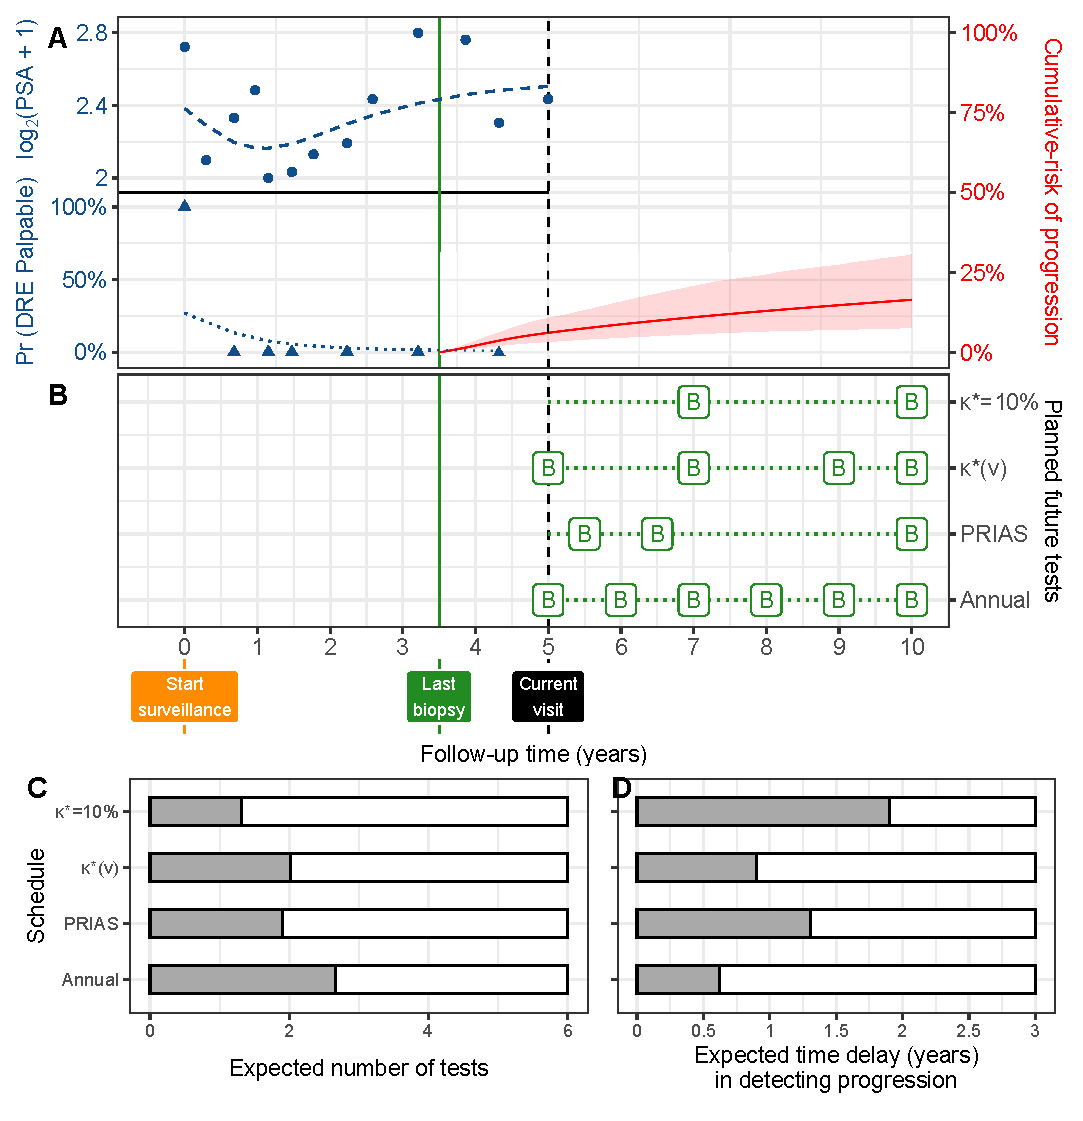
\includegraphics{images/demo_schedule.eps}}
\caption{\textbf{Illustration of personalized schedules for a demonstration PRIAS patient:} In \textbf{Panel~A}: Time of last negative biopsy is year 3.5 (vertical green solid line). Longitudinal data: DRE (blue triangles) and PSA (blue circles). The current visit is year five (vertical black dashed line). The estimated cumulative-risk profile is shown with a solid red line (95\% credible interval is shaded). It is 18.8\% at year ten (horizon). In \textbf{Panel~B}, we visualize different biopsy schedules, with a `B' indicating a biopsy. \textbf{$\kappa=10\%$} and \textbf{$\kappa^*(v)$} are personalized biopsy schedules using a fixed risk threshold of 10\%, and automatically chosen threshold~(\ref{eq:kappa_choice}), respectively. PRIAS and Annual denote the PRIAS biopsy schedule (paragraph~2 of Section~\ref{sec:results}) and annual biopsy schedule. \textbf{Panel~C,D}: For all schedules we calculate the expected number of tests and expected time delay in detecting progression if the patient progresses before year ten. Since a recommended minimum gap of one year is maintained between biopsies, maximum possible number of tests are six.  A delay in detecting progression of up to three years may not lead to adverse outcomes~\citep{carvalho}. }\label{fig:demo_schedule}
\end{figure}